\documentclass[12pt]{article}
\usepackage{amsmath}
\usepackage{fancyhdr}
\usepackage{geometry}
\usepackage{parskip}
\usepackage{pdfpages}
\usepackage{graphicx}
\usepackage{mathtools}

\graphicspath{{./}}
\geometry{letterpaper, portrait, margin=1in}
\setlength{\parindent}{0pt}

\fancyhf{}
\pagestyle{fancy}

\lhead{Math 252 Take-home Quiz}
\rhead{Solomon Greenberg}

\newcommand{\me}{\mathrm{e}}
\newcommand{\dx}{\mathrm{d}x}
\newcommand{\du}{\mathrm{d}u}
\newcommand{\dtheta}{\mathrm{d}\theta} \newcommand{\md}{\mathrm{d}}
\DeclarePairedDelimiter\abs{\lvert}{\rvert}%
\DeclarePairedDelimiter\norm{\lVert}{\rVert}%

% Swap the definition of \abs* and \norm*, so that \abs
% and \norm resizes the size of the brackets, and the 
% starred version does not.
\makeatletter
\let\oldabs\abs
\def\abs{\@ifstar{\oldabs}{\oldabs*}}

\let\oldnorm\norm
\def\norm{\@ifstar{\oldnorm}{\oldnorm*}}
\makeatother


\begin{document}
    \pagenumbering{gobble}
    \newpage
    \pagenumbering{arabic}

    % \paragraph*{6.1:} 2, 3, 6, 9, 15, 17, 21, 22, 23, 26, 27, 29, 30
    % \paragraph*{6.2:} 1, 2, 3, 5, 9, 14, 16, 20, 21, 25, 26, 28, 31, 33

    
    3D printer nozzle for 3 mm diameter filament with a rough approximation of screw threading\\
    Used Ti-$n$spire to solve integrals, and Wolfram Alpha when my calculator was out of arm's reach\\

    1 graph unit = 1 cm\\
    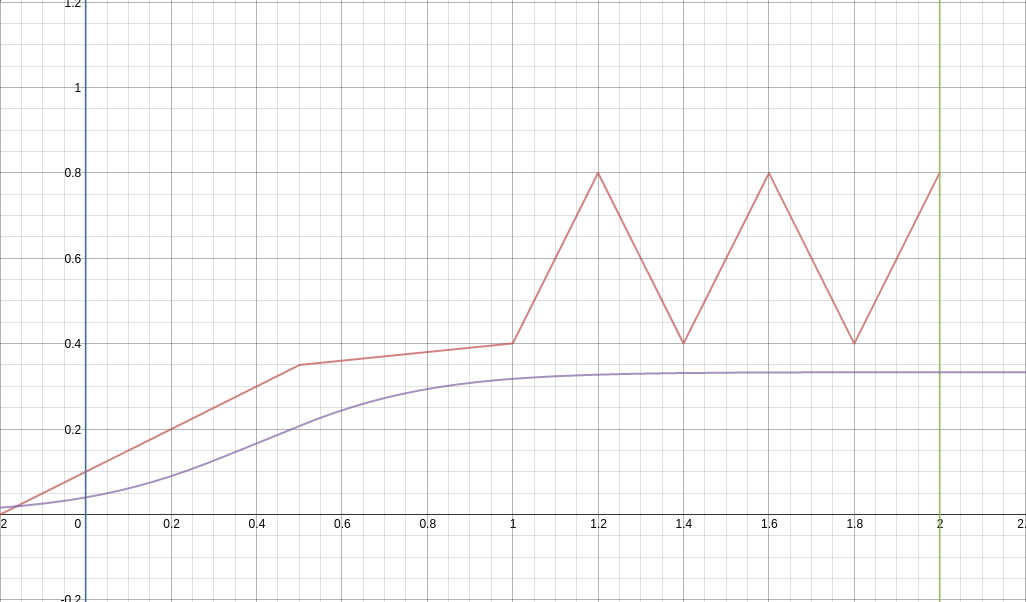
\includegraphics[scale=.3]{2016-06-06-162120_1026x602_scrot.png}\\


    $y = {x < 0.5: 0.5x + 0.1, x < 1: 0.1x + 0.3, x < 2: \frac{2}{5\pi}\cdot\arcsin{(\sin{(4\pi\cdot x - \frac{3\pi}{2})})} + 0.6}$\\
    $y = \frac{1}{3(1 + \me^{-(5x-2)})}$\\

    Area under piecewise function:\\
    $\int_{0}^{0.5}\! \frac{1}{2}x + \frac{1}{10}\,\dx = 0.1125$\\
    $\int_{0.5}^{1}\! \frac{1}{10}x + \frac{3}{10}\,\dx = 0.1875$\\
    $\int_{1}^{2}\!    \frac{2}{5\pi}\arcsin{(\sin{(4\pi\cdot x - \frac{3\pi}{2})})} + 0.6    \,\dx = 0.6$\\
    Total: $0.9$\\\\

    Area under sigmoid function:\\
    $A(x) = \int\!\frac{1}{3(1 + \me^{-(5x-2)})}$
    $= \frac{1}{15}\cdot \ln{(\me^{5x} + \me^2)}$\\
    $A(x)|_{0}^{2} = \frac{1}{15}\cdot \ln{(\me^{10} + \me^2)} - \frac{1}{15}\cdot \ln{(\me^{0} + \me^2)}$\\
    $= \frac{1}{15} \cdot (2 - \ln{(1 + \me^2)} + \ln{(1 + \me^8)})$\\
    $\approx 0.525$\\\\

    Area between functions:\\
    $0.375$\\\\

    Volume:\\
    $\int_{0}^{0.5}\! 2\pi((0.5x + 0.1) - (\frac{1}{3(1 + \me^{-(5x-2)})}))\,\dx$\\
    $\approx 0.352$\\
    $\int_{0.5}^{1}\! 2\pi((0.1x + 0.3) - (\frac{1}{3(1 + \me^{-(5x-2)})}))\,\dx$\\
    $\approx 0.309$\\
    $\int_{1}^{2}\!   2\pi((\frac{2}{5\pi}\cdot\arcsin{(\sin{(4\pi\cdot x - \frac{3\pi}{2})})} + 0.6) - \frac{1}{3(1 + \me^{-(5x-2)})}) \,\dx$\\
    $\approx 1.70$\\
    Total $= 0.352 + 0.309 + 1.7 = 2.361 $cm$^3$\\\\


    Use for shape: Nozzle for 3D printer hotends; attaches to heater block and melts a filament of plastic 3mm in diameter and extrudes it at 0.4mm.\\\\

    Material of choice: Brass.\\
    Density of brass: $8.7\,\,\, \mathrm{g}/\mathrm{cm}^3$\\
    Total weight of object: $8.7 * 2.361 = 20.5407 g$\\\\
    
    Sketch:


\thispagestyle{fancy}

\end{document}

